\documentclass[12pt, notitlepage]{article}	
\usepackage{sample}% use style file "sample.sty" in cwd

\begin{document}

%%%%% Title
\title{\latex Typesetting}
\author{Asako Mikami}
\date{\today}
\maketitle

\begin{abstract}
This is a sample document created in a \latex text editor. It demonstrates some of \latex syntax necessary to write reproducible research papers such as 
\begin{enumerate*}[label =\alph*)]
\item writing mathematics in \latex; 
%\item inserting and executing R codes with \knitr chunks; 
%\item inserting figures from files and displaying figure output from R code; 
%\item formatting regression output from R into a table using \stargazer package; 
\item inserting footnotes; 
\item typesetting hyperlinks to navigate the document; 
\item adding appendix section; 
\item adding bibliography at the end of the document. 
\end{enumerate*}
The document uses a \texttt{.sty} file named \texttt{sample.sty}, and a \texttt{.bib} file named \texttt{sample.bib}. Both files are stored in the same directory as this file. 
\end{abstract}

%%%%%%%%%%%%%%%%%%%

\begin{notes}
Meta comments are displayed in blue. They can be hidden by 
\begin{enumerate}[label=\arabic*.)]
\item opening the style file associated with this document, \texttt{sample.sty}, located in the current directory,
\item commenting the line, \verb|\includecomment{notes}|, 
\item uncommenting the line, \verb|\excludecomment{notes}|.
\end{enumerate}
\end{notes}



\section{Probability: random variable and cdf}

\begin{notes}
Begin a section by typing \verb|\section{}| with the section title inside the brackets.
\end{notes}

\begin{notes}
Here is a paragraph containing \textit{italics}, inline math delimited by $\texttt{\$ \ldots \$}$, and a footnote with two hyperlinks, one to the Appendix section and another to a web page.
\end{notes}
\\

We say $X = X(\omega)$ is a \textit{random variable} that maps an outcome/event $\omega$ in sample space $\Omega$ to a real number.\footnote{A more technical definition states that $X$ is a measurable function mapping an \textit{event space} $\mathcal{F}$ to $\mathbb{R}$, which implies that not all outcomes are events and not all events are outcomes. See Appendix \ref{measure} and \href{https://stats.stackexchange.com/questions/199280/why-do-we-need-sigma-algebras-to-define-probability-spaces}{this discussion} on StackExchange for the motivation behind conceptualizing probability as a measure.} For example if we have a sample space $\Omega = \{ \text{success}, \text{fail} \}$, then we can map $\Omega$ to $\mathbb{R}$ by coding $X = 1$ when the outcome is a success and $X=0$ when the outcome is a failure. In short, a random variable is a coding scheme.



\begin{notes}
The next passage contains a displayed math delimited by \texttt{$\$\$ \ldots \$\$$} and lists. For numbered lists, use the environment \verb|\begin{enumerate}...\end{enumerate}|. For a bullet lists, use the environment \verb|\begin{itemize}...\end{itemize}|. The lists are formatted to reduce empty space by setting the spacing parameters globally in \texttt{sample.sty} as follows:
\begin{verbatim}
\setlist{topsep=0pt, itemsep = 0pt, leftmargin=50pt}
\end{verbatim}
See \href{https://tex.stackexchange.com/a/300512}{this helpful StackExchange post} for what these parameters mean.
\end{notes}
\\

Say we want to make a statement about the probability of an event $\{\omega \in \Omega | X(\omega) \leq x \}$ for some real number $x$. Such a statement is called a \textit{cumulative distribution function}, denoted $F(x)$ or $F_X(x)$ where 
        $$F(x) = F_X(x) = P(\{X \leq x\}) = P( \{ \omega \in \Omega, X(\omega) \leq x \}).$$ 
Mathematically, $P$ is a special function called a \textit{probability measure} and therefore has the following properties called \textit{Kolmogorov axioms}:
        \begin{enumerate}[label=\arabic*.)]
        \item $0 \leq P(A) < \infty$ for all events $A$;
        \item for a countable sequence of disjoint events $A_1, A_2, \ldots$, $P(\bigcup \limits_{i=1}^\infty A_i) = \sum_{i=1}^\infty P(A_i)$;
        \item $P(\Omega) = 1$.
        \end{enumerate}
Kolmogorov axioms imply the following results.
	\begin{enumerate}[label=\alph*)]
	\item $P(\varnothing) = 0$\footnote{This is one instance where an outcome and an event are not the same because $\varnothing$ cannot an element of $\Omega$ and is not an \textit{outcome}. However, we can still define probabilities for an 		\textit{event}.}
	\item $0 \leq P(A) \leq 1$ for all events $A \in \omega$.
	\item If $A \subseteq B$, then $P(A) \leq P(B)$.
	\item For events $A$ and $B$, $P(A \cup B) = P(A) + P(B) - P(A \cap B)$.  \label{demoivre}
	\end{enumerate}


\begin{notes}
I changed the list label to appear as "a.), b.), c.)" by changing the default numeric label to alphabetic like so.
	\begin{verbatim}
	\begin{enumerate}[label=\alph*)]
	\end{enumerate}
	\end{verbatim}
I also like my numeric labels to appear as "1.), 2.), 3.)" instead of the default, "1., 2., 3.", so I use \verb|[label=\arabic*.)]|.
\end{notes}
\\

Let's prove \ref{demoivre} for exercise. 
\begin{proof}
Assume that $A$ and $B$ are nonempty events where $A \subseteq B$. By the first Kolmogorov axiom, we know that $0 \leq P(A), P(B) < \infty$. If $A \subset B$, then $B/A$ and $A$ are disjoint and their union is $B$. By the second axiom, $P(B) = P((B/A) \cup A) = P(B/A) + P(A)$. Therefore, $P(A) \leq P(B)$.
\end{proof}


\begin{notes}
The \texttt{amsmath} package comes with \texttt{proof} environments:
	\begin{verbatim}
	\begin{proof}
	\end{proof}
	\end{verbatim}
\end{notes}

Using these properties of $P$, we can also derive the following three properties for cumulative distribution function, $F$.
	\begin{itemize}
	\item $F$ is nondecreasing, i.e. $F(x) \leq F(y)$ for all $x < y$.
	\item $\lim_{x \to - \infty}F(x) = 0$ and $\lim_{x \to \infty}F(x) = 1$
	\item $F$ is right continuous, i.e. $\lim_{h \to 0} F(x+h) = F(x)$.
	\end{itemize}
Let's prove the first one for exercise.
\begin{proof}
Assume that $x < y$. Then it must be that $\{X \leq x \} \subset \{X \leq y\}$. By the property we proved above, $P(X \leq x) \leq P(Y \leq y)$. Therefore by the definition of cdf, $F(x) \leq F(y)$.
\end{proof}




\section{Famous distributions}

Notes on notation: I use $p(k)$ for probability mass function and $f(x)$ for probability density function. I use $x$ for real numbers, and $k$ for natural numbers. $\mathbb{I}_{A}$ is an indicator function where 
	$$\mathbb{I}_{A} = \mathbb{I}_{A}(x) = \begin{cases}
											1 & \quad \text{if $x \in A$} \\
											0 & \quad \text{if $x \notin A$} \end{cases}.$$


\begin{notes}
As frequently done, I have set up macros in the style file for the expectation and variance symbols. 
        \begin{verbatim}
        \newcommand{\E}{\mathrm{E}\,}
        \newcommand{\Var}{\mathrm{Var}\,}.
        \end{verbatim}
Now the expectation appears as $\E$ instead of $E$ by typing \verb|\E|. Similarly, the variance appears as $\Var$ instead of $Var$ by typing \verb|\Var|. I have \verb|\,| added there to leave some space after the symbol.
\end{notes}


\subsection*{Uniform distribution, $U(a,b)$}

\begin{notes}
Begin an unnumbered subsection by typing \verb|\subsubsection*{}| with the sub-subsection title inside the brackets. If you want it to be numbered, take out the asterik. For any environment that has the option to be unnumbered (such as lists), you can add an asterik to disable the numbering. 
\end{notes}
\\

A random varible $X$ has a (continuous) uniform distribution if it has constant probability over its sample space, $(a, b)$. 
\begin{align*}
f(x) &= \dfrac{1}{b-a}\, \mathbb{I}_{[a,b]} \\
F(x) &= \begin{cases} 0 & x \leq a \\
                x & a < x < b \\
                1 & x \geq b \end{cases} \\
\E[X] &= \dfrac{a+b}{2}, \quad  \Var(X) = \dfrac{(b-a)^2}{12}
\end{align*}

\subsection*{Normal distribution, $\mathit{N}(\mu, \sigma^2)$}
The bell curve that is observed in \href{https://galtonboard.com/probabilityexamplesinlife}{more places} than you'd think. $X \sim N(\mu, \sigma^2)$ is a normal distribution where $\E[X] = \mu$ and $\Var(X) = \sigma^2$. 
\begin{align*}
f(x) = \dfrac{1}{\sqrt{2\pi \sigma^2}} \exp \Big\{ - \dfrac{(x-\mu)^2}{2\sigma^2} \Big\} \, \mathbb{I}_\mathbb{R}
\end{align*}

\subsection*{Exponential distribution, $\rm{Exp}(\beta)$}
Let $X \sim \rm{Exp}(\beta)$ be a random variable describing the waiting time between events that occur at a constant rate. Then $X$ is said to have an exponential distribution where $\E[X] = \beta$. 
\begin{align*}
f(x) &= \dfrac{1}{\beta} \exp \Big\{ - \dfrac{x}{\beta} \Big\}\mathbb{I}_{[0, \infty)} \\
F(x) & = 1 - \exp \Big\{ - \dfrac{x}{\beta} \Big\} \\
\E[X] &= \beta, \quad \Var(X) = \beta^2
\end{align*}

\subsection*{Bernoulli distribution, $\rm{Ber}(p)$}
Let $X$ describe a one-trial experiment whose outcome can be a success with probability $p$ or a failure with probability $1-p$. Let $X(\text{success}) = 1$ and $X(\text{failure}) = 0$. 
\begin{align*}
p(k) & = P(X=k) = p^k (1-p)^{1-k} \mathbb{I}_{\{0,1\}} \\
\E[X] & = p, \quad \Var(X) = p(1-p)
\end{align*}

\subsection*{Binomial distribution}
A binomial distribution $X \sim \rm{bin}(n, p)$ models an experiment with $n$ trials with $p$ probability of success per trial. Alternatively, it can be modeled as a sum of $n$ independent and identical Bernoulli trials with $p$ probability of success. 
\begin{align*}
P(X=k) & = \binom{n}{k}p^k (1-p)^{n-k}\mathbb{I}_{\{k \leq n\}}\\
\E[X] & = np, \quad \Var(X)  = np(1-p)
\end{align*}


\subsection*{Poisson distribution, $\rm{Poisson}(\lambda)$}
Suppose we want to describe the number of plane crashes that occur in a year. Intuitively, a binomial distribution would make sense. But for rare events where there is a large number of $n$ (number of flights per year) and a small probability of success $p$ (the relative frequency of a plane crash in a year), a Poisson distribution is a good approximation and may be more practical as it uses the average number of successes as the parameter. 
\begin{align*}
p(k) &= P(X =k) = \dfrac{\lambda^k e^{-\lambda}}{k!}\mathbb{I}_{\mathbb{N}_0} \\
\E[X] &= \lambda, \quad \Var(X) = \lambda
\end{align*}



%%%%%%%%%%%%%%%%%%%%%%%%%%%%%%%%%%
\newpage 
\appendix 

\begin{notes}
Use \verb|\appendix| command to begin appendix. 
\end{notes}


\section{Motivation for a measure theory-based probability} \label{measure}

\begin{notes}
I have created a hyperlink to this appendix section by adding \verb|\label{measure}| next to the section tag. I can refer to this section by writing \verb|\ref{measure}|. 
\end{notes}
\\

The goal of a probability measure theory is to unify the discrete and continous cases as the two cases do not parallel each other nicely. In an introductory probability textbook such as \cite{ross}, students first learn that a random variable $X$ may be associated with either a discrete sample space (i.e. the sample space $\Omega$ is countable) or a continuous sample space (i.e. the sample space $\Omega$ is uncountable). Next, they define a probability mass function (pmf) for a discrete r.v. and a probability density function (pdf) for a continuous random variable. At this point, only the pmf actually expresses probability. In order to make a probability statement for a continuous r.v., we need to get to the cumulative distribution function (cdf). This is the first instance where the two cases are not congruent. Second, unlike the relationship between pdf and cdf, where the former is the derivative of the latter and the latter is the integral of the former, the relationship between the pmf and the cdf is not one of a derivative and an antiderivative. The following figure attempts to illustrate the situation. 

\begin{figure}[h!]
\center
\caption{The discrete case and the continuous case do not parallel each other.}
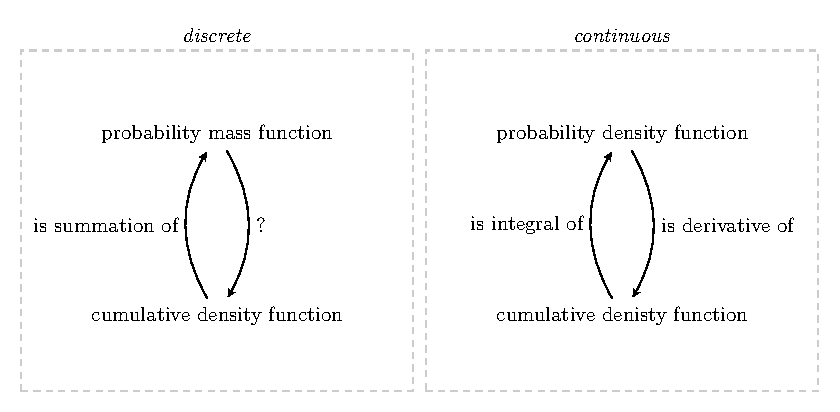
\includegraphics{fig/tikz_graph.pdf}
\end{figure}

A measure theory-based probability solves these inconsistencies. By defining probability as a measure on a measurable set, regardless of whether our random variable is discrete or continuous, it becomes mathematically possible to state that the pdf (pmf) is the derivative of the cdf and that the cdf is the integral of the pdf (pmf). 


\section{How to get help on \latex}

{\LARGE Google it.}\\

There are many ebooks, books, and websites out there illustrating the A to Z of \latex syntax. None of them are short, nor is reading through any of them actually helpful for learning to write in \latex. If you have any question about how to do something in \latex, or in any programming language for that matter, then google it. Chances are that somebody else has already asked the question on \href{https://tex.stackexchange.com/}{Tex StackExchange} and that one of the answers will be the right fit for you. Even when you encounter errors, copy-paste the error message and you'll find a solution on \href{https://tex.stackexchange.com/}{Tex StackExchange}. 

\section{How to get better at \latex}

{\LARGE Practice.}\\

The best way to get better at \latex is to stop using Microsoft Word and do more writing on a \latex text editor. Write your notes in \latex.\footnote{Here are some examples of what I practiced: \href{https://drive.google.com/file/d/0B1KGXZttjtvpZ21OeTE2RW4xLUU/view?usp=sharing}{my probability notes},  \href{https://drive.google.com/drive/folders/0B1KGXZttjtvpd2xHaU9WcFN2OFk}{my game theory notes}.} Write your paper in \latex. Write your CV in \latex. Write your presentation slides in \latex. Look up how you can do something on \latex by googling it and try it out. 


\newpage




\begin{notes}
Use \verb|\printbibliography| command to insert a bibliography. In the style file, I have the following lines specifying that I want the \texttt{biblatex} package to write my bibliography in author-year format with the  \texttt{biber} engine as my \texttt{.bib} processor.
	\begin{verbatim}
	\usepackage[backend=biber, style=authoryear, citestyle=authoryear]{biblatex}
	\addbibresource{sample}
	\end{verbatim}
The \texttt{.bib} file stores all my bibliography entries. You can find a \texttt{bibtex} formatted citation by googling the work you want to cite on \href{https://scholar.google.com/}{Google Scholar}. For example, the entry for \cite{ross} looks like this:
	\begin{verbatim}
	@book{ross,
  		title={A first course in probability},
  		author={Ross, Sheldon},
  		year={2014},
  		publisher={Pearson}
	}
	\end{verbatim}
\end{notes}

\printbibliography



\end{document}
